%%%%%%%%%%%%%%%%%%%%%%%%%%%%%%%%%%%%%%%%%
%
% (c) 2022 by Jennifer Laaser
%
% This work is licensed under the Creative Commons Attribution-NonCommercial-ShareAlike 4.0 International License. To view a copy of this license, visit http://creativecommons.org/licenses/by-nc-sa/4.0/ or send a letter to Creative Commons, PO Box 1866, Mountain View, CA 94042, USA.
%
% The current source for these materials is accessible on Github: https://github.com/jlaaser/pogil-polymers
%
%%%%%%%%%%%%%%%%%%%%%%%%%%%%%%%%%%%%%%%%%

\renewcommand{\figpath}{content/polymchem/livingpolyms/ringopening/figs}
\renewcommand{\labelbase}{ringopening}

\begin{activity}{Ring-Opening Polymerizations}

\begin{instructornotes}
	This activity introduces students to concepts related to ring-opening polymerizations.
	
	After completing this activity, students will be able to:
	\begin{enumerate}
		\item \dots
	\end{enumerate}
	
	\subsection*{Activity summary:}
	\begin{itemize}
		\item \textbf{Activity type:} Learning Cycle
		\item \textbf{Content goals:} Ring-opening polymerizations
		\item \textbf{Process goals:} %https://pogil.org/uploads/attachments/cj54b5yts006cklx4hh758htf-process-skills-official-pogil-list-2015-original.pdf
			\begin{itemize}
				\item Reading and interpreting reaction mechanisms
				\item Interpreting mathematical equations
				\item Oral and written communication of reasoning
			\end{itemize}
		\item \textbf{Duration:} 45 minutes, including class discussion
		\item \textbf{Instructor preparation required:} none beyond knowledge of relevant content
		\item \textbf{Related textbook chapters:}
			\begin{itemize}
				\item \emph{Polymer Chemistry} (Hiemenz \& Lodge): section \dots
			\end{itemize}
		%\item \textbf{Facilitation notes:}
		%	\begin{itemize}
		%		\item \dots
		%	\end{itemize}
	\end{itemize}
	
\end{instructornotes}


\begin{model}[Ring-Opening Polymerization]
	\label{\labelbase:mdl:ROP}

	Ring-opening polymerizations are polymerizations in which a cyclic (ring-shaped) monomer is opened up to form a linear segment of the polymer backbone, as shown below:
	
	\centerline{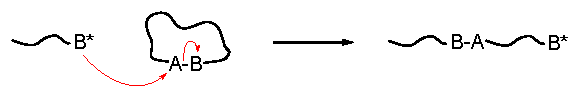
\includegraphics[width=0.8\textwidth]{\figpath/Model1_ROP_general}}
	
	Here, B* denotes the active functional group on the end of the growing polymer chain which is able to attack the A-B bond in the cyclic monomer.
	
	%A specific example of a ring-opening polymerization that you have seen in an earlier activity is anionic polymerization of ethylene oxide, shown below:
	
	%SCHEME
	
\end{model}


\begin{ctqs}

	\question Is the mechanism shown above better described as a chain-growth polymerization or a step-growth polymerization?  Explain your group's reasoning in 1-2 complete sentences.
			
				\begin{solution}[1in]
				\end{solution}

	\question Consider the changes in bonding that occur during this propagation reaction.
	
		\begin{enumerate}
		
			\item Is there any \emph{net change} in the number of A-B bonds present in the reaction mixture during this propagation step?
			
				\begin{solution}[0.5in]
				\end{solution}
	
			\item Is there any \emph{net change} in the number of B* reactive sites present in the reaction mixture during this propagation step?
			
				\begin{solution}[0.5in]
				\end{solution}
	
			\item Based on your answers to the previous questions, do you expect changes in the chemical bonding to contribute significantly to the enthalpy of this reaction? Briefly explain your group's reasoning.
			
				\begin{solution}[1.25in]
				\end{solution}
						
		\end{enumerate}
	
	\question Next, consider the changes in entropy that occur during this reaction.
	
		\begin{enumerate}
			
			\item Does the \textit{translational} freedom of the monomer increase or decrease during this propagation step?  %Briefly explain your group's reasoning.
			
				\begin{solution}[0.5in]
				\end{solution}
			
			\item Does the \textit{conformational} freedom of the monomer increase or decrease during this propagation step?  %Briefly explain your group's reasoning.
			
				\begin{solution}[0.5in]
				\end{solution}
			
			\item Based on your answers to the previous parts of this question, do you expect the overall entropy of the system to increase or decrease during this propagation step?  Briefly explain your group's reasoning.
			
				\emph{Hint: if your answers to parts (a) and (b) were different, which one do you think will be the bigger contribution?}
			
				\begin{solution}[1.5in]
				\end{solution}
			
		\end{enumerate}
		
	\question Finally, consider the changes in the \emph{bond angles} that occur during this propagation reaction.
	
		\begin{enumerate}
		
			\item The structures of cyclopropane and cyclobutane are shown below:
			
				\centerline{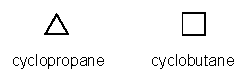
\includegraphics[width=0.4\textwidth]{\figpath/Model1_cyclicmolecules}}
				
				How do the bond angles in these molecules compare to the bond angles you would expect in a linear alkane?
			
				\begin{solution}[2in]
				\end{solution}
				
			\item Based on your answer to the previous question, do you expect ``opening up'' a cyclic molecule to form a linear molecule to be enthalpically favorable or enthalpically unfavorable?  Briefly explain your group's reasoning.
			
				\begin{solution}[1in]
				\end{solution}
			
		\end{enumerate}
		
	\question Based on your answers to CTQs 1-3, what do you expect is the primary driving force for propagation in a ring-opening polymerization?
			
				\begin{solution}[0.75in]
				\end{solution}

\end{ctqs}

\begin{infobox}

	The \emph{ring strain} of a cyclic molecule can be quantified by comparing the heat of combustion for the cyclic molecule to that expected for a linear alkane of the same length.
	
	The ring strains for several small cyclic alkanes are tabulated below:
	% numbers from: https://chem.libretexts.org/Courses/Siena_Heights_University/SHU_Organic_Chemistry_I/3%3A_Chapter_3_Conformations_and_Cycloalkanes/3.04%3A_Stability_of_Cycloalkanes_-_Ring_Strain
	\begin{center}
	\begin{tabular}{lcc}
		\hline		
		Molecule & \ce{CH2} units & Ring Strain (kcal/mol)\\\hline
		Cyclopropane & 3 & 27.6\\
		Cyclobutane & 4 & 26.4\\
		Cyclopentane & 5 & 6.5\\
		Cyclohexane & 6 & 0.0\\
		Cycloheptane & 7 & 6.3\\
		%Cyclooctane & 8 & 9.6%\\\hline
	\end{tabular}
	\end{center}

\end{infobox}

\begin{ctqs}

	\question Based on these numbers, are there any ring sizes for which ring-opening polymerization should \emph{not} be favorable?  Explain your group's reasoning in 2-3 complete sentences.
			
				\begin{solution}[2in]
				\end{solution}

\end{ctqs}

\clearpage
\begin{model}[Ring-Opening Metathesis]
	\label{\labelbase:mdl:ROMP}

	One type of reaction that is frequently used in ring-opening polymerizations is olefin metathesis.
	In an olefin metathesis reaction, two double bonds ``swap partners'', as shown below:
	
	\centerline{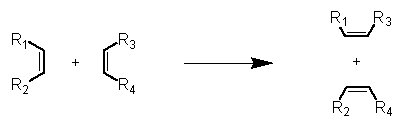
\includegraphics[width=0.6\textwidth]{\figpath/Model2_metathesis_general}}
	
	In polymer chemistry, this process is usually catalyzed by a ruthenium-based catalyst called a Grubbs catalyst.
	
\end{model}

\begin{ctqs}
	
	\question Predict the product of the following metathesis reaction: \label{\labelbase:ctq:metathesis1}
	
		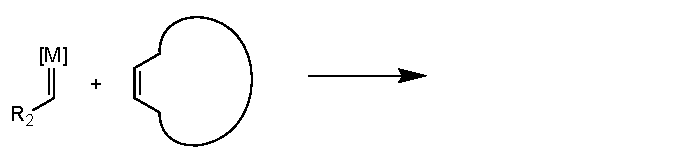
\includegraphics[width=0.5\textwidth]{\figpath/Model2_ROMP_general}
		
		\emph{Note: here, [M] indicates the location of the metal center of the catalyst.}
		
	\question Explain, in 1-2 complete sentences, why olefin metathesis reactions using cyclic molecules can be used to form polymer chains.
			
				\begin{solution}[1.5in]
				\end{solution}
	
	%\question Based on the structures you drew in \ref{\labelbase:ctq:metathesis1}, would you categorize this polymerization as a chain-growth or a step-growth polymerization?  Explain your group's reasoning in 1-2 complete sentences.
	
	\question What type of characteristic bond appears in the backbone of polymers made using this method?
			
				\begin{solution}[0.5in]
				\end{solution}
	
	\clearpage
	\question Propose the structure of the monomer that must have been used to form the following polymer:
	
	\centerline{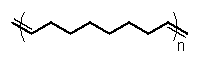
\includegraphics[width=0.25\textwidth]{\figpath/Model2_polycyclooctene}}
			
				\begin{solution}[1in]
				\end{solution}
	
	\question Predict the structure of the polymer that would be formed in a ring-opening metathesis polymerization of norbornene, shown from two angles below:
	
	\centerline{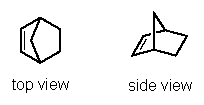
\includegraphics[width=0.3\textwidth]{\figpath/Model2_norbornene}}
			
				\begin{solution}[1in]
				\end{solution}
	
\end{ctqs}


\begin{model}[Polylactide]
	\label{\labelbase:mdl:PLA}

	Another common polymer made by ring-opening polymerization is polylactide (PLA).  The mechanism by which a lactide monomer is added to the polymer chain is shown belw:
	
	\centerline{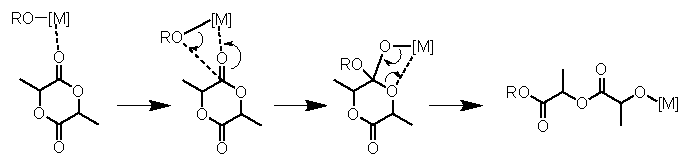
\includegraphics[width=0.7\textwidth]{\figpath/Model3_PLA}}
	
	Here, \ce{[M]} is the metal center of an inorganic catalyst such as tin octoate (\ce{Sn(C8H15O2)2}).
	
\end{model}

\begin{ctqs}
	
	\question Briefly describe what happens to each of the following during the course of this reaction:
	
		\begin{enumerate}
			\item monomer:
			
				\begin{solution}[0.5in]
				\end{solution}
			
			\item catalyst:
			
				\begin{solution}[0.5in]
				\end{solution}
				
		\end{enumerate}
		
	\question Based on the mechanism shown in Model \ref{\labelbase:mdl:PLA}, why do you think this is referred to as a ``coordination-insertion'' polymerization?
			
				\begin{solution}[1in]
				\end{solution}
	
	\question The mechanism shown in Model \ref{\labelbase:mdl:PLA} is a chain-growth polymerization.  However, the resulting polymer could also be prepared \emph{via} a step-growth polymerization as well.
	
		\begin{enumerate}
			\item Propose the structure of the monomer (or monomers) that would be needed to prepare polylactide via a step-growth polymerization.
			
				\begin{solution}[1.5in]
				\end{solution}
			
			\item Based on what you remember about the molecular weight distributions of polymers produced by step-growth polymerization, why do you think that most commercial suppliers of PLA prepare it by the chain-growth mechanism shown in Model \ref{\labelbase:mdl:PLA} instead?  Explain your group's reasoning in 2-3 complete sentences.
			
				\begin{solution}[1.5in]
				\end{solution}
		\end{enumerate}
	
\end{ctqs}




%\begin{exercises}

%	\exercise \dots
	
%\end{exercises}


%\begin{problems}
%
%	\problem First exercise
%	\problem Second exercise
%	
%\end{problems}


	
\end{activity}